\documentclass[11pt]{article}
\usepackage[a4paper,margin=1in]{geometry}
\usepackage{fourier} % Fourier font
\usepackage{xcolor}
\usepackage{tikz}
\usepackage[most]{tcolorbox}
\usepackage{amsthm, amsmath, amssymb}
\usepackage{enumitem}
\usepackage[hyphens]{url}
\usepackage{hyperref}
\usepackage[nameinlink,noabbrev]{cleveref}
\usepackage{titling} 

% Dark mode colors
\definecolor{bgcolor}{HTML}{FFFFFF}
\definecolor{textcolor}{HTML}{1E1E1E}
\definecolor{defcolor}{HTML}{E86873}
\definecolor{thmcolor}{HTML}{0A9396}
\definecolor{lemcolor}{HTML}{34EB52}
\definecolor{corcolor}{HTML}{9B4AF7}
\definecolor{probcolor}{HTML}{EE9B00}
\definecolor{excolor}{HTML}{0C00F5}

% Background and text color
\pagecolor{bgcolor}
\color{textcolor}

% No paragraph indentation
\setlength{\parindent}{0pt}
\setlength{\parskip}{0.7em}

% Theorem box styles
\tcbset{
  enhanced,
  colback=bgcolor,
  colframe=thmcolor,
  coltext=black,
  coltitle=white,
  fonttitle=\bfseries,
  boxrule=0.7pt,
  left=1em,
  right=1em,
  top=0.7em,
  bottom=0.7em,
  before skip=10pt,
  after skip=10pt,
}

% Theorem environments with colored boxes
\newtcbtheorem[number within=section]{thm}{Theorem}{
  colframe=thmcolor, colback=thmcolor!15!bgcolor
}{thm} % The 'thm' here is the *prefix* for the label

\newtcbtheorem[number within=section]{defn}{Definition}{
  colframe=defcolor, colback=defcolor!15!bgcolor
}{def} % The 'def' here is the *prefix* for the label

\newtcbtheorem[number within=section]{lem}{Lemma}{
  colframe=lemcolor, colback=lemcolor!15!bgcolor
}{lem}

\newtcbtheorem[number within=section]{cor}{Corollary}{
  colframe=corcolor, colback=corcolor!15!bgcolor
}{cor}

\newtcbtheorem[number within=section]{prob}{Problem}{
  colframe=probcolor, colback=probcolor!15!bgcolor
}{prob}

\newtcbtheorem[number within=section]{ex}{Example}{
  colframe=excolor, colback=excolor!15!bgcolor
}{ex}

% Proof environment 
\renewenvironment{proof}[1][\proofname]{%
  \par\pushQED{\qed}\normalfont\topsep6pt \trivlist
  \item[\hskip\labelsep\itshape #1.]\ignorespaces
}{%
  \popQED\endtrivlist\addvspace{6pt}
}

% Cleveref name formats for tcolorbox environments
\crefname{thm}{theorem}{theorems}
\Crefname{thm}{Theorem}{Theorems}

\crefname{def}{definition}{definitions}
\Crefname{def}{Definition}{Definitions}

\crefname{lem}{lemma}{lemmas}
\Crefname{lem}{Lemma}{Lemmas}

\crefname{cor}{corollary}{corollaries}
\Crefname{cor}{Corollary}{Corollaries}

\crefname{prob}{problem}{problems}
\Crefname{prob}{Problem}{Problems}

\crefname{ex}{example}{examples}
\Crefname{ex}{Example}{Examples}

\usepackage{graphicx}

\title{\huge{ELE201 Semester Project}}
\author{\LARGE{Thobias Høivik}}
\date{}

\begin{document}
\maketitle

\newpage
\tableofcontents

\newpage
\section{Introduction}
In this project we use the STM32 microcontroller along with analog 
sensors 
to gather data that we analyze for statistical and informational 
randomness, 
with the goal of evaluating how feasible such a setup is as a 
hardware-based true random number generator (TRNG). 
The data will be sent via serial connection to a computer 
to analyze the quality of the data.

We will combine theory from information theory, probability, 
signal processing, and networking to assess both the quality of 
randomness 
and how such a system could integrate into a distributed architecture.

We will discuss:
\begin{itemize}
    \item Theoretical background on randomness and entropy.
    \item Implementation and data transfer.
    \item Statistical analysis and randomness testing.
    \item Viability discussion and possible improvements.
    \item Network design for scaling such systems.
\end{itemize}

\newpage
\section{Theory}
\subsection{Randomness and Entropy}
Randomness can be defined both in a statistical and algorithmic sense. 
A sequence is considered random if it is unpredictable and lacks 
compressible structure.

\begin{defn}{Shannon Entropy}{}
Given a discrete random variable $X$ that takes values in $\chi$ with 
probability distribution $p:\chi \to [0,1]$, its entropy is
$$
    H(X) = - \sum_{x \in \chi} p(x) \log_2 p(x).
$$
\end{defn}

Entropy measures the uncertainty of a random variable. 
For a binary sequence, $H(X) = 1$ indicates perfectly balanced and 
maximally unpredictable bits.

Intuitively, high entrop should mean unpredictable bits, while 
low entropy should mean that the bits are structured and predictable.
This sounds very good for our purposes, but if we look at 
a string like "$010101010101\dots$", where we alternate 
$0$s and $1$s, we get a shannon entropy of $1$ which is as high 
as we can go. However, this string of bits very clearly has 
a predictable structure, which entropy alone cannot take into account.

\begin{defn}{Min-Entropy}{}
The min-entropy of a random variable $X$ is
$$
H_{\text{min}}(X) = -\log_2 \left(\max_x p(x)\right),
$$
representing the worst-case predictability of any outcome.
\end{defn}

\subsection{True vs. Pseudo Randomness}
A pseudo-random number generator (PRNG) produces deterministic 
sequences 
from an initial seed, while a true random number generator (TRNG) 
relies 
on physical entropy. 
For hardware-based RNGs, ensuring unbiased and unpredictable output 
requires:
\begin{itemize}
    \item High-quality analog entropy sources.
    \item Proper sampling rates and whitening.
    \item Statistical post-processing.
\end{itemize}

\subsection{Statistical Tests of Randomness}
We use the NIST SP 800-22 statistical test suite as a theoretical 
foundation. The most relevant tests include:
\begin{itemize}
    \item Frequency (Monobit) Test
    \item Runs Test
    \item Autocorrelation Test
    \item Approximate Entropy Test
    \item Linear Complexity Test
\end{itemize}
Each of these tests returns a $p$-value indicating how likely the 
observed sequence could occur under true randomness.

\newpage
\subsection{Theoretical Modeling of Analog Noise} 
To justify that the least significant bits of our ADC contains 
randomness, we model the analog sensor output as a combination of 
deterministic signal and noise: 
\[ 
    V_{\text{ADC}}(t) = V_{\text{Signal}}(t) + V_{\text{Noise}}(t)
\]

\begin{itemize}
    \item \(V_{\text{Signal}}\) represents the slowly varying, 
        predictable component (e.g. ambient light level in the case 
        of photoresistor). 
    \item \(V_{\text{Noise}}\) represents the unpredictable physical 
        noise (thermal-, shot noise, quantization error, 
        sensor-specific noise).
\end{itemize}

We assume that $V_{\text{Noise}}$ is a zero-mean gaussian random 
variable: 
\[ 
    V_{\text{Noise}}(t) \sim \mathcal N(0, \sigma^2) 
\]

This assumption is fairly reasonable for electronic circuits, 
where thermal noise and shot noise dominate at small scales 
(citation desparately needed).

The \textbf{ADC quantization} transforms the continuous voltage 
into discrete levels: 
\begin{align*}
    X = \text{ADC}(V_{\text{ADC}}) \in \{0,1,\dots,2^{12}-1\}
    \\
    (\text{in the case where we sample at } 12-\text{bits})
\end{align*}


\begin{figure}[h]
    \centering
    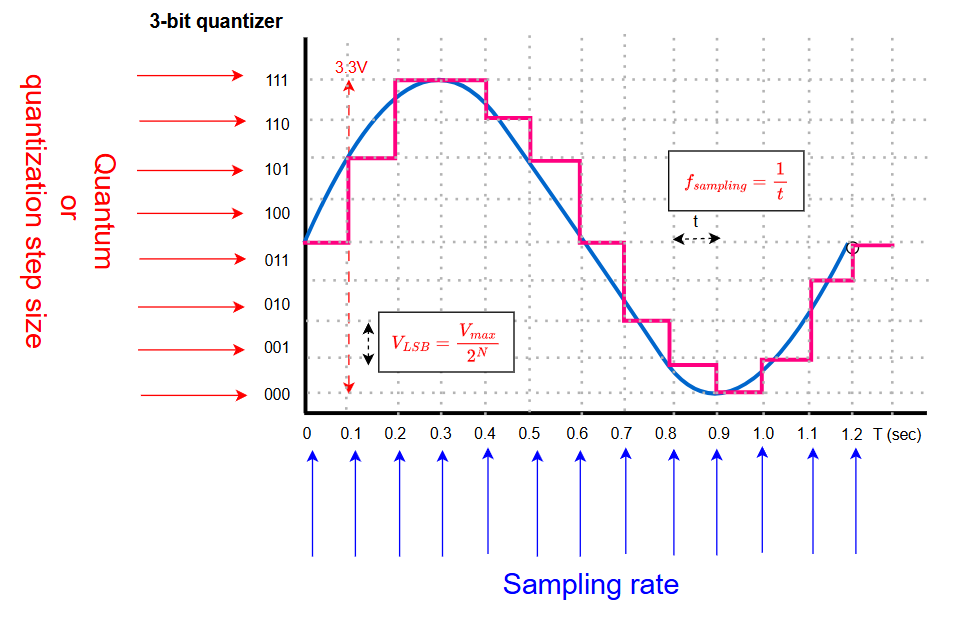
\includegraphics[width=0.8\linewidth]{./images/quantization.png} 
    \caption{Quantization of analog signal.}
    \label{fig:quantization} 
\end{figure}
(NOTE: REMEMBER TO ASK Gizem HOW TO CITE THIS IMAGE)

If we denote the least significant bit (LSB) of \(X\) 
by \(\text{LSB}(X)\), then under the Guassian noise model, 
the probability that the LSB is \(1\) is approximately 
\[ 
    P(\text{LSB}(X) = 1) \approx \frac{1}{2} 
\]

This is because, if we consider a single interval 
\([k\Delta V, (k+1)\Delta V)\), if $V_\text{Noise}$ is uniformly 
distributed across this interval, then the probability that the 
that we round to $(k+1)\Delta V$ or $k\Delta V$ is equal and one 
of these will be odd. Hence there is a roughly $1/2$ chance 
that the least significant bit will be a $1$.


\newpage
\section{Implementation}
\subsection{Hardware Setup}
We will use the STM32 microcontroller, connected to one or more analog 
sensors. Candidate sensors include:
\begin{itemize}
    \item Microphone or sound sensor.
    \item Light-dependent resistor (LDR).
    \item Temperature sensor.
\end{itemize}

The microcontroller samples the analog voltage via the ADC and 
stores or 
streams the digital values over a serial or network interface.
For now we will be working with a light sensor, sampling 
at $12$ bits and looking at bits in the lower end of the 
range as they will be most prone to interference and noise.

\subsection{Data Transmission}
Data is transmitted from the STM32 to a computer for analysis. 
This can be done using:
\begin{itemize}
    \item UART/Serial connection.
    \item Ethernet or WiFi (via ESP module or similar).
\end{itemize}

For our purpose of analyzing the data for randomness a serial 
connection will do and we will use UART, sending the data 
to a computer where we can analyze the data.

\subsection{Processing}
Our goal is to transform the raw data stream 
(which is \textbf{biased} and \textbf{predictable}) into a shorter, 
statistically perfect random stream.

\begin{enumerate}
    \item Raw Bit Extraction 
        \begin{itemize}
            \item \textbf{Technique:} Only use the least significant
                bits of the ADC output. 
            \item The LSBs are dominated by the desired random noise 
                sources and are less influenced by the much larger 
                and more predictable signal 
                (e.g. light level in the case of a light sensor).
                Thus the MSBs should be discarded entirely as they 
                should exibit fairly low entropy.
        \end{itemize}

    \item Entropy Conditioning (Post-Processing) 
        Since the LSBs will more than likely still contain 
        residual bias and correlation we require a powerful 
        \textbf{Entropy Extractor} for cryptographic quality.
        \begin{itemize}
            \item \textbf{XOR Folding:}
                XOR a bit with one a few steps behind. 
                E.g. $\text{Bit}_{\text{Out}} = 
                \text{Bit}_i \oplus \text{Bit}_{i-N}$, 
                where $N$ is chosen to be slightly larger than 
                the observed correlation length.

            \item \textbf{Cryptographic Hash Extractor 
                (NIST SP 800-90B):}
                Collect a large buffer of $L$ raw bits. 
                Estimate $H_{\text{min}}$ per bit. Take the buffer, 
                and hash it (e.g. SHA-256) to produce a fixed-length 
                output.

                Ths downside with this approach is that we have to 
                sample many times to get a sufficiently large buffer.
        \end{itemize}
\end{enumerate}



\newpage
\section{Results and Analysis}

\subsection{Network Design}
A possible setup:
\begin{itemize}
    \item Each microcontroller is connected to a local router.
    \item A dedicated subnet for sensor nodes (e.g., 192.168.10.0/24).
    \item Central analysis server on a separate subnet.
\end{itemize}

\subsection{Subnetting and Addressing}
We show how to subnet the network efficiently:
\begin{itemize}
    \item Example: dividing a /24 into four /26 subnets.
    \item Assigning IP ranges for sensors, analysis nodes, and administration.
\end{itemize}

\subsection{Data Security and Transmission Integrity}
We briefly discuss:
\begin{itemize}
    \item Packet integrity verification (CRC or checksum).
    \item Optional encryption for data in transit.
    \item Synchronization and time-stamping for accurate sampling.
\end{itemize}

\newpage
\section{Conclusion}
We summarize:Fundamentals of Precision ADC
Noise Analysis
\begin{itemize}
    \item Theoretical feasibility of analog-sensor-based TRNGs.
    \item Experimental results and limitations.
    \item Potential for distributed entropy networks.
\end{itemize}

\subsection{Future Work}
\begin{itemize}
    \item Hardware whitening circuits and amplification.
    \item FPGA or ASIC implementations.
    \item Scaling to larger networks and entropy pooling.
\end{itemize}

\newpage
\section*{References}

NOTE: Some stuff I've looked at 
\begin{verbatim}
Harvesting_Entropy_for_Random_Number_Generation_fo.pdf 

https://nvlpubs.nist.gov/nistpubs/Legacy/SP/nistspecialpublication800-22r1a.pdf 
(NIST-800-22)

A Mathematical Theory of Communication
By C. E. SHANNON (Entropy)

Fundamentals of Precision ADC
Noise Analysis
Texas Instruments (Noise is inherent in all electrical systems)
\end{verbatim}


\end{document}

